\documentclass[12pt]{article} \setlength{\oddsidemargin}{0in}
\setlength{\evensidemargin}{0in} \setlength{\textwidth}{6.5in}
\setlength{\parindent}{0in} \setlength{\textwidth}{16cm}
\setlength{\topmargin}{1in} \addtolength{\topmargin}{-1.5in}
\setlength{\textheight}{23cm} \setlength{\parskip}{0.75cm}

% Brackets
\usepackage{mathtools}
\DeclarePairedDelimiter\ceil{\lceil}{\rceil}
\DeclarePairedDelimiter\floor{\lfloor}{\rfloor}

% Tikz settings
\usepackage{tikz}
\usetikzlibrary{trees}
\usetikzlibrary{positioning}
\usetikzlibrary{calc}
\definecolor{mypurple}{cmyk}{0.6,0.4,0.1,0}
\definecolor{myred}{cmyk}{0,0.3,0.3,0}
\usetikzlibrary{fit,shapes.misc}

% Typesetting options
\usepackage[utf8]{inputenc}
\usepackage{fancyvrb}
\usepackage{amsmath,amsfonts,amssymb}
\usepackage[english]{babel}
\usepackage[autostyle, english = american]{csquotes}
\usepackage[none]{hyphenat}
\usepackage{url}

% For MATLAB/Mathematica files
\usepackage{listings}
\usepackage{matlab-prettifier}
\lstloadlanguages{[5.2]Mathematica}

% Numbering Options
\usepackage{enumitem}
\setlist[1]{label=(\alph*)} % Sets level 1 default format to (a)
\setlist[2]{label=(\roman*)} % Sets level 2 default format to (i)

% Other useful packages
\usepackage{multicol}
\usepackage{qtree}
\usepackage{float}
\usepackage{adjustbox}

\graphicspath{ {images/} }


% Make sectioning a breeze
\makeatletter\renewcommand\section{
	\@startsection{section}{1}{\z@}
    {0ex}
    {1ex}
    {\ifnum \thesection > 1
    	\newpage
    \fi
    \large\textbf{Problem }\large\textbf}}

\title{CSCI 3104 Algorithms Homework 10}

\begin{document}

\noindent CSCI 3104 Spring 2018 \hfill Problem Set 10\\
\textbf{Cole Schlisner} (04/26)\\
\noindent\rule{\linewidth}{0.5pt}

\section{}
\textit{(15 pts total) A matching in a graph $G$ is a subset $E_M \subseteq E(G)$ of edges such that each vertex touches at most one of the edges in $E_M$. Recall that a bipartite graph is a graph $G$ on two sets of vertices, $V_1$ and $V_2$, such that every edge has one endpoint in $V_1$ and one endpoint in $V_2$. We sometimes write $G = (V_1, V_2; E)$ for this situation. For example:}

\begin{table}[H]
\centering
\begin{tikzpicture}[font = \normalsize, scale = 1.5, clip = {0 0 2cm 0}]
\node (V1) at (0,0)  {$V_1:$};
\node (1)  at (1,0)  {1};
\node (2)  at (2,0)  {2};
\node (3)  at (3,0)  {3};
\node (4)  at (4,0)  {4};
\node (5)  at (5,0)  {5};
\node (6)  at (6,0)  {6};
\node (V2) at (0,-1) {$V_2:$};
\node (7)  at (1,-1) {7};
\node (8)  at (2,-1) {8};
\node (9)  at (3,-1) {9};
\node (10) at (4,-1) {10};
\node (11) at (5,-1) {11};

\path[-] (1) edge (8)
         (2) edge (7)
         (3) edge (10)
         (4) edge (9)
         (6) edge (11);

\path[dotted] (2) edge (8)
                  edge (9)
              (3) edge (7)
                  edge (11)
              (4) edge (8)
                  edge (10)
              (5) edge (9)
                  edge (11);
\end{tikzpicture}
\end{table}

\textit{The edges in the above example consist of all the lines, whether solid or dotted; the solid lines form a matching.\\
The bipartite maximum matching problem is to find a matching in a given bipartite graph $G$, which has the maximum number of edges among all matchings in $G$.}

\begin{enumerate}
\item\textit{Prove that a maximum matching in a bipartite graph $G = (V_1, V_2; E)$ has size at most $\min\{|V_1|,|V_2|\}$.}

If: $|V_1| > |V_2|$ then for every vertex v $\in$ $V_2$ there is a corresponding vertex u $\in$ $V_1$. If a matching is made between all pairs of (v, u) then: (1) there are $|V_2| = \min\{|V_1|,|V_2|\}$ edges in the matching and (2) by the pigeonhole principle there will be $|V_1| - |V_2|$ verticies in $V_1$ that cannot be matched with any verticies in $V_2$ as they have already been matched. 

\item\textit{Show how you can use an algorithm for max-flow to solve bipartite maximum
matching on undirected simple bipartite graphs. That is, give an algorithm which, given an undirected simple bipartite graph $G = (V_1, V_2; E)$:}
\begin{enumerate}[label = (\arabic*)]
\item\textit{constructs a directed, weighted graph $G'$ (which need not be bipartite) with weights $w : E(G') \rightarrow \mathbb{R}$ as well as two vertices $s; t \in V(G')$,}
\item\textit{solves max-flow for $(G',w), s, t$, and}
\item\textit{uses the solution for max-flow to find the maximum matching in $G$. Your algorithm may use any \texttt{max-flow} algorithm as a subroutine.}
\end{enumerate}
\pagebreak
The next two pages contain python ($>= 2.7$) code for generating a matching for an arbitrary bipartite graph. The MaxMatching function is a working implementation of the algorithm in question. If the code is run it will generate a matching for the example.
The algorithm:\\
\begin{enumerate}
\item creates a new graph g'
\item adds all edges, verticies from the input graph to g'
\item makes all edges from $V_1$ to $V_2$ directed edges ($V_1$ $\rightarrow$ $V_2$)
\item adds two verticies s and t to the graph
\item connects s $\rightarrow$ {$V_1$} and {$V_2$} $\rightarrow$ t
\item adds 2 weights to each edge representing the initial residual flow capacity (1) and initial flow (0)
\item solves the Max Flow problem on g' (using Ford-Fulkerson)
\item constructs a map of $u \in V_1$ to $v \in V_2$ such that there is a saturated edge (u,v) in g' . This is the matching. 
\pagebreak
\end{enumerate}
\begin{verbatim}
# assume g is a dict of adjacency lists of a simple undirected bipartite graph
# g[1] = the adjacency list for vertex 1 , containing names of other verticies
def MaxMatching(g):
  # gflow is a dictionary of {'node name' : [list of edges from this node]}
  # each edge will be represented as a 3-tuple: (dest vertex, capacity, flow)
  gflow = {n+1 : [] for n in range(len(g))}
  v1 = set()
  v2 = set()
  # add all of the edges from g, add verticies in edges to groups v1 and v2
  # set all residual capacities to 1
  for v in g.keys():
    if v not in v2:
      v1.add(v) 
    for e in g[v]:
      # only add edges from v1 -> v2
      if v in v1:
        gflow[v].append((e, 1, 0))
        v2.add(e)
      else: v1.add(e)
  # fully connect s -> {v1}
  gflow['s'] = [(v, 1, 0) for v in v1]
  # fully connect {v2} -> t
  gflow['t'] = []
  for v in v2:
    gflow[v].append(('t', 1, 0))
  # solve max flow on gflow with Ford-Fulkerson:
  sigma = DFS(gflow, 's', 't')
  while sigma is not None:
    minCap = 10**4
    for n in range(len(sigma)-1):
      for e in gflow[sigma[n]]:
        if e[0] == sigma[n+1] and e[1] < minCap:
            minCap = e[1]
    for n in range(len(sigma)-1):
      for i, e in enumerate(gflow[sigma[n]]):
        if e[0] == sigma[n+1]:
          gflow[sigma[n]][i] = (e[0], e[1]-minCap, e[2]+minCap)
    sigma = DFS(gflow, 's', 't')
  matching = {}
  for v in v1:
    for e in gflow[v]:
      if e[1] == 0: # no residual capacity
        matching[v] = e[0]
  return v1, v2, gflow, matching

# assume gf is a flow graph in the form of a dictionary {'name':[edges]} 
def DFS(gf, s, t):
  pred = {k:None for k in gf.keys()}
  old = {k:False for k in gf.keys()}
  sigma = []
  Q = [s]
  while (len(Q) > 0):
    v = Q.pop()
    if not old[v]:
      old[v] = True
      for e in gf[v]:
        if e[1] > 0: 
        # there is still residual capacity on this edge
          if e[0] == t: 
          # we found a path 
            sigma.insert(0,t)
            p = v
            while p is not None:
              sigma.insert(0,p)
              p = pred[p]
            return sigma
          pred[e[0]] = v
          Q.append(e[0])
  return None

ex = {1:[8], 2:[7,8,9], 3:[10,7,11], 4:[8,9,10], 5:[9,11], 
    6:[11], 7:[2,3], 8:[1,2,4], 9:[2,4,5], 10:[3,4], 11:[3,5,6]}

v1, v2, gf, m = MaxMatching(ex)

print("flow graph:: ")
for k in gf.keys():
  print(" %s : %s"%(k, gf[k]))
print("v1:: %s"% v1)
print("v2:: %s"% v2)
print("Matching:: %s"%m)


\end{verbatim}
\newpage

\item\textit{Show the weighted graph constructed by your algorithm on the example bipartite graph above.}

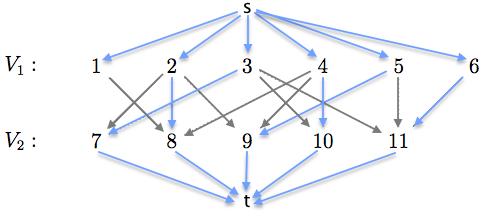
\includegraphics{p1c}

In the directed graph above, the blue edges represent edges with weight 1 (flow=1, residual capacity=0) and the grey edges represent edges with weight 0 (flow=0, residual capacity 1).

\end{enumerate}

\section{}
\textit{(20 pts total) In the review session for his Deep Wizarding class, Dumbledore reminds everyone that the logical definition of NP requires that the number of bits in the witness $w$ is polynomial in the number of bits of the input $n$. That is, $|w| = poly(n)$. With a smile, he says that in beginner wizarding, witnesses are usually only logarithmic in size, i.e., $|w| = O(\log n)$.}
\begin{enumerate}
\item\textit{Because you are a model student, Dumbledore asks you to prove, in front of the whole class, that any such property is in the complexity class P.}

If $|w| = (\log n)$ then enumerating all possible witnesses can be done in polynomial time, thus finding the witness is a P class problem. i.e. $2^{log(n)} = n^{log(2)}$


\item\textit{Well done, Dumbledore says. Now, explain why the logical definition of NP implies that any problem in NP can be solved by an exponential time algorithm.}

There are exponentially many ($2^{n^c}$) possible witnesses when $|w| = poly(n)$, thus they can only be enumerated in exponential time. 

\item\textit{Dumbledore then asks the class: ``So, is NP a good formalization of the notion of problems that can be solved by brute force? Discuss.'' Give arguments for both possible answers.}\\

Yes, because exponential computation can \textit{technically} be done in finite time and space. \\

No, because there are many NP problems that cannot \textit{practically} be done. i.e. cannot be done with all of the computing power on earth before the heat death of the universe.

\end{enumerate}

\section{}
\textit{(30 pts total) The Order of the Phoenix is trying to arrange to watch all the corridors in Hogwarts, to look out for any Death Eaters. Professor McGonagall has developed a new spell, Multi-Directional Sight, which allows a person to get a 360-degree view of where they are currently standing. Thus, if they are able to place a member of the Order at every intersection of hallways, they'll be able to monitor all hallways. In order not to spare any personnel, they want to place as few people as possible at intersections, while still being able to monitor every hallway. (And they really need to monitor every hallway, since Death Eaters could use Apparition to teleport into an arbitrary hallway in the middle of the school.) Call a subset $S$ of intersections ``safe,'' if, by placing a member of the Order at each intersection in $S$, every hallway is watched.}
\begin{enumerate}
\item\textit{Formulate the above as an optimization problem on a graph. Argue that your formulation is an accurate reflection of the problem. In your formulation, show that the following problem is in NP: Given a graph $G$ and an integer $k$, decide whether there a safe subset of size $\leq k$.}

The corresponding optimization problem on a graph G = (V,E) would be finding a set of verticies W $\subseteq$ V such that for all (u,v) $\in$ E, $u \in W$ or $v \in W$. 

This problem is analogous if the edges are considered 'corridors' and verticies considered 'intersections'; a vertex $v$ is only reachable from another vertex $u$ iff there is an edge between them or a series of edges that begin at $u$ and end on $v$. This is the same for real corridors and intersections. \\

A non-deterministic (lucky) algorithm that chooses the optimal intersection to cover at every step would need at most $k$ steps to decide, and checking whether all corridors are covered after each step is O(E) (this could be done in O(1) with caching). Thus our lucky algorithm would take at worst $O(kE)$ = linear time to solve the problem, so this problem is in NP. 


\item\textit{Consider the following greedy algorithm to find a safe subset:}
\begin{verbatim}
S = empty
mark all hallways unwatched
while there is an unwatched hallway
    pick any unwatched hallway; let u,v be its endpoints
    add u to S
    for all hallways h with u as one of its endpoints
        mark h watched
    end
end
\end{verbatim}
\textit{Although this algorithm need not find the minimum number of people needed to cover all hallways, prove that it always outputs a safe set, and prove that it always runs in polynomial time.}\label{s:SafeProof}

The work of this algorithm is done in the \textit{while} loop on line 3. This loop checks if the amount of unwatched hallways (which I will call $u$) is greater than zero. Before the loop enters, all hallways are unwatched. During the loop, at least one hallway becomes watched (i.e. $u$ is strictly decreasing). This is because we pick an unwatched hallway on line 4, select one of its endpoints, and then mark it as watched on line 7 along with every other hallway that is connected to the selected endpoint. Because $u$ decreases by $\ge$ 1 every loop, $u$ will be equal to zero after $O(E)$ loops.

This means that, (A) the algorithm always runs in $O(E^2)$ time (because we presumably scan through all of E on line 6) and (B) once the loop exits there are necessarily no more unwatched hallways, and every (watched) hallway is connected to a vertex in S, so S is always a safe set. 

\item\textit{Note that, in order to be polynomial-time, an algorithm for this problem cannot simply try all possible subsets of intersections. Prove why not.}

There are $2^V$ possible subsets of the vertex set $V$ (for every $v \in V$, you can either add it to the subset or not). $O(2^n)$ is exponential-time, not polynomial time.

\item\textit{Give an example where the algorithm from \ref{s:SafeProof} outputs a safe set that is strictly larger than the smallest one. In other words, give a graph $G$, give a list of vertices in the order in which they are picked by the algorithm, and a safe set in $G$ which is strictly smaller than the safe set output by the algorithm.}

G: 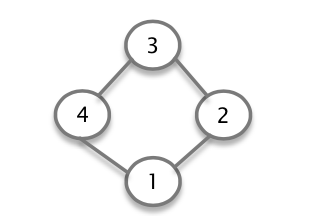
\includegraphics[width=3.4cm,height=3cm]{p3d} \\

S picked by algorithm: $\{1,2,3\}$\\

Smallest safe set: $\{1,3\}$

\pagebreak

\item\textit{Consider the following algorithm:}
\begin{verbatim}
S = empty
mark all hallways unwatched
while there is an unwatched hallway
    pick any unwatched hallway; let u,v be its endpoints
    add u,v to S
    for all hallways h with u or v one of their endpoints
        mark h watched
    end
end
\end{verbatim}
\textit{Although this algorithm need not find the minimum number of people needed to cover all hallways, prove that it always outputs a safe set, and prove that it always runs in polynomial time.}\label{s:SafeProof2}

The work of this algorithm is done in the \textit{while} loop on line 3. This loop checks if the amount of unwatched hallways (which I will call $u$) is greater than zero. Before the loop enters, all hallways are unwatched. During the loop, at least one hallway becomes watched (i.e. $u$ is strictly decreasing). This is because we pick an unwatched hallway on line 4, select both of its endpoints, and then mark it as watched on line 7 along with every other hallway that is connected to either of the selected endpoints. Because $u$ decreases by $\ge$ 1 every loop, $u$ will be equal to zero after $O(E)$ loops.

This means that, (A) the algorithm always runs in $O(E^2)$ time (because we presumably scan through all of E on line 6) and (B) once the loop exits there are necessarily no more unwatched hallways, and every (watched) hallway is connected to a vertex in S, so S is always a safe set. 

\item\textit{In any safe set of intersections, each hallway is watched by at least one member of the Order. Use this to show that the algorithm from \ref{s:SafeProof2} always outputs a safe set whose size is no more than twice the size of the smallest safe set. Note: you don't need to know what the smallest safe set is to prove this! All you need is the fact stated here.\\
This is called a ``2-approximation algorithm,'' because it is guaranteed to output a solution that is no worse than a factor of 2 times an optimal solution.}

The algorithm from \ref{s:SafeProof2} adds 2 verticies for each edge (i.e. in the worst case, 2 times the minimum amount required because only 1 vertex is required per edge). In other words, in the worst case the optimal vertex is selected for each edge, along with an extra edge. Since all of the optimal edges (OPT) are included in the safe set (S) returned by the algorithm, the amount of non-optimal edges in S cannot exceed $|S \setminus OPT| = 2*|OPT|$. 

\pagebreak

\item\textit{Does the algorithm from \ref{s:SafeProof} always produce a safe set no bigger than that produced by the algorithm in \ref{s:SafeProof2}? If so, give a proof; if not, give a counterexample. A counterexample here consists of a graph, and for each algorithm, the list of vertices it chooses in the order it chooses them, such that the safe set output by algorithm \ref{s:SafeProof} is at least as large as the safe set output by algorithm \ref{s:SafeProof2}. If you are unable to give either a proof or a counterexample, then for partial credit give a plausible intuitive argument for your answer.}

No. Here's a counterexample: \\

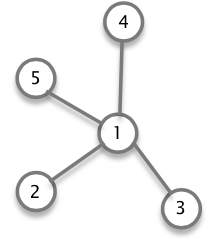
\includegraphics[width=3.4cm,height=3cm]{p3g}

Algorithm \ref{s:SafeProof}: $\{2,3,4,5\}$ \\
Algorithm \ref{s:SafeProof2}: $\{2,1\}$

\item\textit{Compare the greedy algorithm from \ref{s:SafeProof2} with the greedy algorithm from \ref{s:SafeProof}. Show which runs faster asymptotically? Which of these two algorithms would you rather use to solve the Order of the Phoenix's problem and why?}

They have the same running time -- consider the worst case for algorithm \ref{s:SafeProof} in which the amount of watched hallways is only increasing by 1 each loop iteration. This is also the worst case for algorithm \ref{s:SafeProof2}, as we can design a graph like a ring such that the amount of watched hallways only increases by 1 every loop (after the first selection).\\

I would use algorithm \ref{s:SafeProof2} because it is guaranteed to always pick the optimal verticies (resulting in having no more than 2 times the optimal amount of guards), even though it may also pick some non-optimal verticies. This is in contrast to the first algorithm, which has the possibility of picking every non-optimal vertex. \\

(I would actually try to use a greedy algorithm that sorts the verticies by degree and adds them to S in that order until there are no more unwatched edges)

\item\textit{This problem is, in fact, NP-complete. Why does the 2-approximation polynomial-time algorithm from \ref{s:SafeProof2} not show that P=NP?\footnote{Interestingly, it is known that if there were a 1.3606...-approximation algorithm for this problem in polynomial time, then it would follow that P=NP, but that is a very nontrivial theorem. Under a standard complexity-theoretic assumption, even if there were a 1.99999-approximation algorithm in polynomial time, it would follow that P=NP, but this assumption remains a conjecture, and opinion in the research community is divided on whether this conjecture is true or false. We will provide references to these results after the problem set has been handed in.}}

Because it is not efficient. (This is more or less an "I don't know") 

\end{enumerate}

\section{}
\textit{(20 pts extra credit) Every young wizard learns the classic NP-complete problem of determining whether some unweighted, undirected graph $G = (V,E)$ contains a simple path of length at least $k$ (where both $G$ and $k$ are part of the input to the problem), known as the Longest Path Problem. Recall that a simple path is a path $(v_1, v_2, ... , v_\ell)$ where each $(v_i, v_{i+1})$ in the path is an edge, and all the $v_i$ are distinct; its length is $\ell-1$ (=the number of edges in the path).}
\begin{enumerate}
\item\textit{Ginny Weasley is working on a particularly tricky instance of this problem for her Witchcraft and Algorithms class, and she believes she has written down a ``witness'' for a particular input $(G, k)$ in the form of a path $P$ on its vertices. Explain how she should verify in polynomial time whether $P$ is or is not simple path of length  $k$. (And hence, demonstrate that the problem of Longest Path is in the complexity class NP.)}

Verify that for each successive pair of verticies ($v_i$,$v_{i+1}$) $\in P$, the edge ($v_i$,$v_{i+1}$) $\in E(G)$ and $v_i$,$v_{i+1}$ are unique among all verticies in $P$.

\item\textit{For the final exam in Ginny's class, each student must visit the Oracle's Well in the Forbidden Forest. For every bronze Knut a young wizard tosses into the Well, the Oracle will give a yes or no response as to whether, given an arbitrary graph $G$ and an integer $k$, $G$ contains a simple path of length  $k$. Ginny is given an arbitrary graph $G$ and must find the longest simple path in $G$. First, she realizes it would be useful to determine the length of the longest simple path. Describe an algorithm that will allow Ginny to use the Oracle to find the length of the longest simple path in $G$ by asking it a series of questions, each involving a modified version of the original graph $G$ and a number $k$. Her solution must not cost more Knuts than a number that grows polynomially as a function of the number of vertices in $G$. (Hence, prove that if we can solve the Longest Path decision problem in polynomial time, we can solve its optimization problem as well.)}

\begin{verbatim}
def longest-path-len(G):
    let k = V(G).length
    while k > 0:
        if ask-oracle(G,k) = yes:
            return k
        k = k-1
    return "G is not a graph"
\end{verbatim}

\pagebreak

\item\textit{Next, once she knows the length $\ell$ of the longest simple path in $G$, Ginny must use the Oracle to actually find a path of length $\ell$. Describe an algorithm that will allow Ginny to use the Oracle to find the longest simple path in $G$ by asking it a series of questions, each involving a modified version of the original graph $G$ and a number $k$ of her choosing (for each question she can ask about a different graph $G$ and a different number $k$). Her solution must not cost more Knuts than a number that grows polynomially as a function of the number of vertices in $G$. (Hence, prove that if we can solve the Longest Path decision problem in polynomial time, we can solve its search problem as well.)}

\begin{verbatim}
def longest-path(G):
    let P = []
    let k = longest-path-len(G)

    // find all verticies in path
    for u in V(G):
        if ask-oracle({G-u},k) = no:
            P += u

    // place the starting vertex in the first position of P
    for i in [1 .. P.length]:
        isFirst = True
        for v in { P - P[i] }:
            // if there is an edge v->P[i], P[i] is not the first in the path
            if Edge(v, P[i]) in E(G):
                isFirst = False
                break
        if isFirst:
            // swap the elements at locations 1, i in P
            swap(P, 1, i)
            break

    // put path in correct order
    for i in [1 .. P.length]:
        for j in [i+1 .. P.length]:
            if Edge(P[i], P[j]) in E(G):
                swap(P, i+1, j)
                break
    return P
\end{verbatim}

\pagebreak

\end{enumerate}
\section{}
\textit{(20 pts extra credit) Recall that the \texttt{MergeSort} algorithm (Chapter 2.3 of CLRS) is a sorting algorithm that takes $\Theta(n \log n)$ time and $\Theta(n)$ space. In this problem, you will implement and instrument \texttt{MergeSort}, then perform a numerical experiment that verifies this asymptotic analysis. There are two functions and one experiment to do this.}
\begin{enumerate}[label=(\roman*)]
\item\textit{\texttt{MergeSort(A, n)} takes as input an unordered array $A$, of length $n$, and returns both an in-place sorted version of $A$ and a count $t$ of the number of atomic operations performed by \texttt{MergeSort}}.
\item\textit{\texttt{randomArray(n)} takes as input an integer $n$ and returns an array $A$ such that for each $0 \leq i < n$, $A[i]$ is a uniformly random integer between 1 and $n$. (It is okay if $A$ is a random permutation of the first $n$ positive integers; see the end of Chapter 5.3.)}.
\end{enumerate}
\begin{enumerate}
\item\textit{From scratch, implement the functions \texttt{MergeSort} and \texttt{randomArray}. You may not use any library functions that make their implementation trivial. You may use a library function that implements a pseudorandom number generator in order to implement \texttt{randomArray}.
Submit a paragraph that explains how you instrumented \texttt{MergeSort}, i.e., explain which operations you counted and why these are the correct ones to count.} 

I implemented MergeSort as the standard two-function combo: MergeSort(A) being the recursive parent function that splits the list up into two, and Merge(A, i) being the function that sorts while merging two lists. I chose to omit the second argument from the definition of MergeSort to simplify it in exchange for an O(1) cost of getting the length from the supplied list. As far as I'm concerned it is a redundant argument because the information about the array length is already in the array. I first split the list up into two pieces using the standard splice syntax in python, feed those sublists into Mergesort to be sorted, and construct a single list out of them. This makes two sub-list copies (right and left halves) and incurs an O(n/2) cost per copy. Adding the second sorted list to the first costs another O(n/2). This list is then fed into the Merge function along with the index of the midpoint between the two lists. Merge simultaneously iterates through the first and second halves of the list, comparing the next element of each list and adding the minimum of the two to the sorted array sA that is returned. Once an element from either half of the input list is added to sA, the starting index for that list is increased, so the next element will be compared. I excluded all assignements to the operation counter, as it doesn't really matter to the efficiency of Mergesort. 
\pagebreak
\begin{verbatim}
def MergeSort(A):
  t = 0 # not counting ops related to counting ops
  n = len(A) 
  t += 1 # len() on a list is an atomic op
  
  if n == 1:
    return A, t
  
  l = MergeSort(A[:int(n/2)])[0] 
  t += 1 + int(n/2) # assignment + list copy
  
  l.extend(MergeSort(A[int(n/2):])[0]) 
  t += n # copy + extend

  sA, s = Merge(l, int(n/2)) # s = atomic ops in Merge()
  
  return sA, (s+t) 

def Merge(A, m):
  i = 0 
  j = m # start of second sorted half
  sA = []
  t = 3 # assignments, allocation
  while len(sA) < len(A):
    if i < m and j < len(A) and A[i] < A[j]:
      sA.append(A[i])
      i += 1
    elif j < len(A):
      sA.append(A[j])
      j += 1
    elif i < m:
      sA.append(A[i])
      i += 1
    t += 10 # conditions + append + re-assign
  return sA, t

import random as r
def randomArray(n):
  return [r.randint(1,n) for i in range(n)]
\end{verbatim}

\pagebreak

\item\textit{For each of $n = \{2^4,2^5,...,2^{26},2^{27}\}$, run \texttt{MergeSort(randomArray(n),n)} five times and record the tuple $(n, \left<t\right>)$, where $\left<t\right>$ is the average number of operations your function counted over the five repetitions. Use whatever software you like to make a line plot of these 24 data points; overlay on your data a function of the form $T(n) = An\lg n$, where you choose the constant $A$ so that the function is close to your data.\\
Hint: To increase the aesthetics, use a log-log plot.}

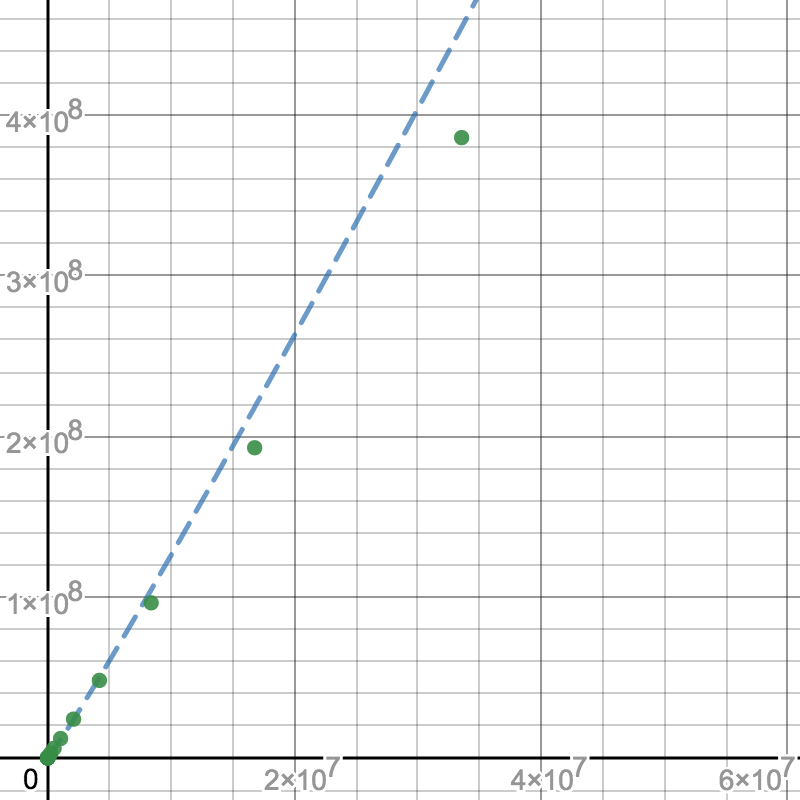
\includegraphics[width=10cm,height=10cm]{p5b} \\

The blue line is $1.8nlogn$

\end{enumerate}


\newpage

\textbf{References} \\
\hrulefill
\begin{enumerate}
  \item CLRS
  \item \url{https://en.wikipedia.org/wiki/Dominating_set}
  \item \url{https://en.wikipedia.org/wiki/Merge_sort}
  \item \url{https://wiki.python.org/moin/TimeComplexity}
\end{enumerate}
\end{document}
